\documentclass[a4paper,12pt]{article}

\usepackage[labelsep=space]{caption}
\usepackage{xltxtra}
\usepackage[lithuanian]{babel}
\usepackage{mathtools}
\usepackage{cite}
\usepackage{verbatim}
\usepackage{subfig}
\usepackage[section]{placeins}

\usepackage{indentfirst}
\usepackage{fullpage}

\usepackage{float}
\usepackage{wrapfig}
\restylefloat{figure}

\usepackage{tikz}
\usetikzlibrary{shapes,arrows}

\begin{document}

\begin{titlepage}

\begin{center}


% Upper part of the page

\textsc{\LARGE Vilniaus Universitetas} \\
\textsc{\LARGE Fizikos Fakultetas} \\
\textsc{\LARGE Kietojo Kūno Elektronikos Katedra}\\[2cm]

\textsc{\Large Vytis Valentinavičius}\\[1.5cm]



% Title

{ \huge \bfseries Difuzijos įtakos krūvininkų pernašai ir rekombinacijai skaičiavimas}\\[1cm]

\textsc{\Large Bakalaurinis baigiamasis darbas}\\[2cm]

% Author and supervisor
\begin{minipage}{0.4\textwidth}
\begin{flushleft} \large
\emph{Katedros vedėjas:} \\
\emph{Darbo vadovas:} \\
\emph{Recenzentas:} \\
\emph{Studentas:} \\
\end{flushleft}
\end{minipage}
\begin{minipage}{0.4\textwidth}
\begin{flushright} \large
prof. K. Arlauskas \\
N. Nekrašas \\
G. Juška\\
V. Valentinavičius \\
\end{flushright}
\end{minipage}



\vfill

% Bottom of the page
{\large 2012 m. Vilnius}

\end{center}

\end{titlepage}
\tableofcontents
\pagebreak

\section{Įvadas}

\paragraph*{Tikslas}
\begin{itemize}
\item Kodėl žmonėms įdomus photo-CELIV?
\item Ką mas pastebėjome nagrinėdami ją anksčiau?
\item Ką reikia padaryti, kad geriau suprastume difuzijos įtaką?
\end{itemize}

Pastaruoju metu sparčiai vystoma nauja mokslo šaka, nagrinėjanti puslaidininkinius organinius darinius. Mokslininkai, kurdami naujas organines medžiagas, didelį dėmesį skiria elektrinių savybių gerinimui.

Organinių medžiagų tyrimui pastaruoju metu itin dažnai naudojama fotogeneruotų krūvininkų ištraukimo tiesine įtampa (photo-CELIV) metodika \cite{juška:155202}. Deja, vienos iš svarbiausių medžiagos charakteristikų, krūvininkų judrio, nustatymui naudojami teoriniai sąryšiai sukurti remiantis modeliais, kuriuose fizikiniai reiškiniai atskirti vienas nuo kito \cite{langevin}. Tuo tarpu organinėse medžiagose išmatuotas krūvininkų judris gali priklausyti nuo elektrinio lauko, prilipimo lygmenų, krūvininkų rekombinacijos ar difuzijos. Akivaizdu, jog tokiais atvejais tikslaus analitinio modelio sudarymas gali būti itin komplikuotas arba netgi neįmanomas, taigi tenka remtis skaitmeniniu modeliavimu.

Šis darbas yra anksčiau rašytuose darbuose \cite{vytis:kursinis, juška:155202} nagrinėtos difuzijos įtakos krūvininkų pernašai ir eksperimentiniams rezultatams tęsinys. Pastaruosiuose darbuose nagrinėta fotogeneruotų krūvininkų ištraukimo tiesine įtampa metodika (photo-CELIV), taigi neatsitiktinai šiame darbe bus nagrinėjama paviršiuje koncentruotų krūvininkų dinamika. Dėmesys sutelktas į difuzijos įtaką rekombinacijai ir iš to sekančius rezultatus.
Skaičiavimai atlikti su autoriaus sukurta programa \cite{vytis:openreadings2010}. Platesnis programos aprašymas ir programos kodas patalpintas GitHub svetainėje \cite{doi@github}.

\paragraph{Darbo tikslai}
\begin{itemize}
\item Naudojant skaitmeninį modeliavimą nustatyti eksperimentines sąlygas, kurioms esant negalima atmesti difuzijos įtakos gautiems rezultatams.
\item Naudojant skaitmeninį modeliavimą paaiškinti difuzijos įtaką rekombinacijai.
\end{itemize}

\pagebreak

 
\section{Naudojamas teorinis modelis}

Šiame darbe naudojamas modelis pasirinktas atsižvelgiant į vyksmus netvarkiose organinėse medžiagose, tačiau bandyta neapriboti modelio viena medžiagų klase. Taigi modelyje yra įskaitomi difuzijos ir krūvininkų dreifo bei rekombinacijos reiškiniai kiek įmanoma bendresniu pavidalu. 

\subsection{Uždavinio diskretizavimas}

Daugelio realių photo-CELIV eksperimentų bandiniai yra “sumuštinio” pavidalo. Tokius bandinius galima redukuoti į vienmates parametrų pasiskirstymo funkcijas. Dėl to šiame darbe bandinys modeliuojamas kaip vienmatė krūvininkų tankio funkcija:
\begin{equation}
\begin{array}{c}
n=n(x)\\
p=p(x)
\end{array}
\end{equation}
Čia \(n,p\) atitinkamai neigiamų krūvininkų ir teigiamų krūvininkų tankis. Taip pat supaprastinome uždavinį teigdami, jog dielektrinė skvarba yra konstanta.
\begin{equation}
\varepsilon(x,E)=\textit{const}
\end{equation}
Modeliuojant skaitmeniškai būtina tolydinį tankių pasiskirstymą suskaidyti į diskretinį. Tai atlikta visą bandinį sudalinus į \(M\) narvelių kuriuose krūvininkų kiekis būtų lygus:
\begin{equation}
\begin{array}{c}
N_i = \frac { n(x_i) + n(x_i+1)}{2} \Delta x S\\
P_i = \frac { p(x_i) + p(x_i+1)}{2} \Delta x S
\end{array}
\end{equation}
Čia \(x_i= \Delta x i\), kur \(i \in [0,M)\) narvelio numeris, \(\Delta x\) narvelio plotis, \(S\) bandinio plotas (žr. \ref{fig:diskretizavimas}~pav.).
\begin{figure}
  \centering
    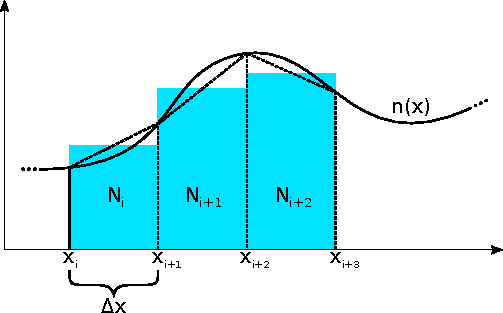
\includegraphics[scale=0.9]{./media/pdf/il1}
  \caption{Tankio diskretizavimas}
  \label{fig:diskretizavimas}
\end{figure}

Diskretizavimas visada įneša netikslumų, tačiau, didindami sudalinimų skaičių \(M\) galime pasiekti norimą skaičiavimo tikslumą (vėliau parodysime, kaip nuo \(M\) priklauso uždavinio trukmė).
Skaičiuojama laikinė sistemos evoliucija, tad reikalingas ir laiko diskretizavimas:
\begin{equation}
\begin{array}{c}
N_i = N_i(t_j) \equiv N_{i,j}\\
P_i = P_i(t_j) \equiv P_{i,j}\\
t_j = t_{j-1} + \Delta t_j
\end{array}
\end{equation}
Čia \(j\) - yra simuliacijos žingsnis, \(\Delta t_j\) - kintamas laiko žingsnis, \(t_j\) diskretizuoto laiko momentas, priklausantis nuo kintamo laiko žingsnio.

\subsection{Dreifas}

Modelyje krūvininkų pernaša vyksta dėl dreifo ir difuzijos. Dreifas skaičiuojamas naudojantis Drūdės modeliu \cite{ashcroft}, kuris teigia, jog esant elektriniam laukui kietajame kūne krūvininkai juda greičiu proporcingu lauko stipriui. Šis greitis vadinamas dreifo greičiu $v_d$.
\begin{equation}
	v_d= \mu E
\end{equation}
	
Čia \(\mu\) krūvininkų judris, \(E\) elektrinio lauko stipris.
Naudojantis greičio išraiška galime užrašyti srovės tankį:
\begin{equation} \label{eq:tankis}
	j_d = v_d n e = \mu n e E
\end{equation}
Iš kitos pusės, laikydamiesi anksčiau aprašyto diskretizavimo, srovės tankį pagal apibrėžimą galime užrašyti taip:
\begin{equation} \label{eq:pokytis}
\frac{\Delta N_{i,j}}{\Delta t_j} \frac{e}{S}=(j_d)_{i,j}
\end{equation}
	
Krūvininkai, išėję iš narvelio per laiko žingsnį \(\Delta t_j\) sukuria srovę. Nuo krūvininkų ženklo ir išėjimo krypties priklauso sukurtos srovės kryptis. Simuliacijos metu laikoma, jog teigiamą srovę sukuria neigiami krūvininkai judantys koordinatės indekso $i$ didėjimo kryptimi.
Taigi suminis srovės tankis laiko momentu \(t_j\) yra toks:
\begin{equation}
j_d(t_j)= \sum_{i=0}^{M} (j_d)_{i,j}
\end{equation}
	

Naudodamiesi diskretizuota \eqref{eq:pokytis} išraiška ir srovės tankio \eqref{eq:tankis} išraiška galime užrašyti:
\begin{equation}
\frac{\Delta N_{i,j}}{\Delta t_j} = \frac{\mu N_{i,j} E_j}{\Delta x}
\end{equation}
Tuo tarpu elektrinis laukas bandinyje susideda iš išorinio ir vidinio elektrinių laukų:
\begin{equation}
\vec{E} = \vec{E}_{in} + \vec{E}_{ex}
\end{equation}

Mūsų nagrinėjamu atveju išorinį elektrinį lauką kuria įtampa prijungta prie bandinio kontaktų, taigi jį galima laikyti nepriklausoma laikine funkcija:
\begin{equation}
	E_{ex}=f(t)
\end{equation}
Vidinio lauko stipris turi būti apskaičiuojamas naudojant Puasono lygtį:
\begin{equation}
	E_{in}(x)=-\frac{e}{\varepsilon \varepsilon_0 S} \int_{0}^{x} x(n-p)dx
\end{equation}
Matome, jog vidinis elektrinis laukas paverčia nagrinėjamą problemą į integro-diferencialinę lygtį.
Pereiname prie diskretinės išraiškos:
\begin{equation}
	E_{in,i}=-\frac{e}{\varepsilon \varepsilon_0 S } \sum_{k=0}^{i}(N_k-P_k)
\end{equation}
Čia \(E_{in,i}\) lauko stipris kuriamas \(i\)-tojo narvelio.



\subsection{Difuzija}

Esant krūvininkų tankio erdviniam pasiskirstymui, vyksta krūvininkų difuzinė pernaša. Pagal Fiko dėsnį:
\begin{equation}
	\frac{\partial n}{\partial t}=-D \frac{\partial^2 n}{\partial x^2}
\end{equation}
Čia \(D\) difuzijos konstanta.

Krūvininkų tankio antrą išvestinę pagal koordinatę keičiame į gretimų narvelių krūvininkų skaičiaus skirtumą:
\begin{equation} \label{eq:difuzija}
\frac{\Delta N_{i,j}}{\Delta t_j} = -D \frac{(N_{i,j-1}-N_{i-1,j-1})}{(\Delta x)^2} - D \frac{(N_{i,j-1}-N_{i+1,j-1})}{(\Delta x)^2}
\end{equation}
Šiame modelyje naudojamės Einšteino sąryšiu difuzijos koeficientui suskaičiuoti:
\[
	D=\frac{k_B T \mu }{e}
\]	
Formulėje~\eqref{eq:difuzija} užrašyti du nariai norint atskirti krūvininkus judančius tarp \(N_{i-1}\) ir \(N_i\) narvelių, bei krūvininkus judančius tarp \(N_i\) ir \(N_{i+1}\) narvelių. Taip atskirta nes, skirtingai nuo dreifo, vieno ženklo krūvininkai gali išeiti abiem kryptimis.
Kadangi formulė \eqref{eq:difuzija} aprašo bendrą krūvininkų skaičiaus kitimą narvelyje dėl difuzijos, sumuojant difuzinę srovę naudojamas tik teigiamas pokytis, tai yra, norint išvengti dvigubos sumos, sumuojami tik iš narvelio išeinantys krūvininkai. Sumavimas analogiškas dreifo srovės komponentės skaičiavimui:
\begin{equation}
	\frac{\Delta N_{i,j}}{\Delta t_j} \frac{e}{S}=(j_c)_{i,j}
\end{equation}
\begin{equation}
	j_c(t_j)= \sum_{i=0}^{M} (j_c)_{i,j}
\end{equation}
	
\subsection{Rekombinacija}

Kietajame kūne egzistuoja keli krūvininkų rekombinacijos mechanizmai, pavyzdžiui monomolekulinė rekombinacija, bimolekulinė ar trimolekulinė (Ožė) rekombinacija. Organiniuose puslaidininkiuose monomolekulinė rekombinacija vyksta, kai judantį krūvininką pagauna rekombinacijos centras. Toks mechanizmas priklauso tik nuo vienų krūvininkų tankio, laikant jog centrų kiekis yra daug didesnis ir nekinta vykstant rekombinacijai. Tuo tarpu esant palyginamiems abiejų ženklų krūvininkų tankiams arba kai krūvininkai juda nestipriame potenciniame lauke, rekombinacijos sparta ima priklausyti nuo abiejų ženklų krūvininkų tankių. Būtent tokios sąlygos yra aprašomame modelyje. Organinėse medžiagose bimolekulinės rekombinacijos vyravimą lemia dar ir tai, kad pernaša vyksta šuoliais arba krūvininkams tuneliuojant per tarpmolekulinius barjerus. Kitaip tariant krūvininkai yra priversti kurį laiką būti lokalizuoti ties viena molekule, ir tuo metu gali rekombinuoti su kitu atėjusiu krūvininku. Trimolekulinė rekombinacija yra nežymi organiniuose puslaidininkiuose, taigi jos galime nepaisyti \cite{juška:143303,juška:013303}.
Remiantis Lanževeno \cite{langevin} aptartu atveju, efektinė bimolekulinės rekombinacijos sparta yra propocinga krūvinkų judriui:
\begin{equation}
B_L=\frac{e}{\varepsilon \varepsilon_0}(\mu_n+\mu_p)
\end{equation}
Taigi rekombinacijos spartą galime aprašyti taip:
\begin{equation} \label{eq:langevin}
\frac{dn}{dt}=-B_L n p
\end{equation}
Tačiau dažnai eksperimentuose stebimas rekombinacijos spartos neatitikimas su Lanževeno teorine verte \(B_L\). Išmatuota rekombinacijos sparta būna mažesnė už teorinę \cite{juška:155202}. Dėl šio neatitikimo į \eqref{eq:langevin} formulę įvedamas redukcijos faktorius \(\eta\), parodantis kiek kartų rekombinacija silpnesnė už teorinę:
\begin{equation}
	\frac{dn}{dt}=-\eta B_L n p
\end{equation}
Kai kuriais atvejais šis rekombinacijos susilpnėjimas yra naudingas, pavyzdžiui, saulės elementų gamyboje, kur norima naudoti medžiagas su dideliu judriu, tačiau silpna rekombinacija.
Rekombinacijos sparta simuliacijoje valdoma keičiant valdantį parametrą \(\eta\).

\subsection{Šviesos sugertis}

Laisvųjų krūvininkų sukūrimui photo-CELIV metodikoje naudojamas šviesos impulsas. Dėl to pradinis krūvininkų pasiskirstymas yra apskaičiuojamas pagal Beer-Lambert’o taisyklę šviesos sugerčiai:
\begin{equation}
	I(x)=I_0 e^{-\alpha x}
\end{equation}
Čia \(I_0\) šviesos intensyvumas ties bandinio paviršiumi, \(I(x)\) šviesos intensyvumas gylyje \(x\), \(\alpha\) sugerties koeficientas.
Simuliacijoje laikome jog apšviečiama bandinio \(x=0\) ploštuma.

Dažnai vietoje \(\alpha\) naudojamas sugerties profilio parametras \(\alpha d\) kuris priklausomai nuo skaitinės vertės leidžia įvardinti sugerties tipą: \(\alpha d < 1\) sugertis tūrinė, krūvininkai sukuriami beveik vienodai visame tūryje, \(\alpha d > 1\) sugertis paviršinė, beveik visa šviesa sugeriama bandinio paviršiuje. Čia \(d\) yra bandinio storis.
Laikydami, jog generacijos kvantinis našumas yra lygus vienetui, tai yra, jog vienas fotonas sukuria vieną porą krūvininkų, galime užrašyti pradinį generuotų krūvininkų skaičių:
\begin{equation}
	P_0(x) = N_0(x) = \alpha I(x)S
\end{equation}
	
Čia \(\alpha I(x)S\) yra poras kuriančių fotonų skaičius gylyje \(x\).
Taigi pradinės sąlygos priklauso nuo dviejų parametrų: \(I_0\) (šviesos intensyvumo) ir \(\alpha d\) (sugerties profilio). Ankstesniuose skaičiavimuose buvo parodyta šių parametrų įtaka photo-CELIV signalui \cite{juška:155202}.

Programoje generuojamų krūvininkų kiekis valdomas keičiant parametrą \(I_0 S\), o profilis valdomas parametro \( \alpha \).

 
\section{Programa}

\begin{figure}
\centering
% Define block styles
\tikzstyle{decision} = [diamond, draw, fill=blue!20, 
    text width=4.5em, text badly centered, node distance=4cm, inner sep=0pt]
\tikzstyle{block} = [rectangle, draw, fill=blue!20, 
    text width=6em, text centered, rounded corners, minimum height=4em]
\tikzstyle{line} = [draw, -latex', ultra thick]
\tikzstyle{cloud} = [draw, ellipse,fill=red!20, node distance=3cm,
    minimum height=2em]
    
\begin{tikzpicture}[node distance = 4cm, auto]
    % Place nodes
    \node [block] (init) {Simuliacijos būsenos išsaugojimas};
    \node [block, below of=init] (timestep) {\( t_j = t_{j-1} + \Delta t_j\)};
    \node [block, below of=timestep] (calculate) {Naujos būsenos skaičiavimai};
    \node [block, left of=timestep] (change) {\(\Delta t_j = \frac{\Delta t_j}{10}\)};
    \node [block, left of=calculate] (restore) {Atstatome paskutinę sistemos būseną};
    \node [decision, below of=calculate] (check) {Ar pažeisti tikslumo reikalavimai?};
    \node [decision, right of=check, node distance=8cm] (end) {Ar simuliacija baigta?};
    \node [decision, above of=end] (timecheck) {Ar galima atstatyti laiko žingsnį?};
    \node [block, right of=timestep] (backroll) {\(\Delta t_j = 10 \Delta t_j \)};
    \node [block, below of=end] (final) {Pabaiga};

    % Draw edges
    \path [line] (init) -- (timestep);
    \path [line] (timestep) -- (calculate);
    \path [line] (calculate) -- (check);
    \path [line] (check) -| node [near start] {Taip} (restore);
    \path [line] (restore) -- (change);
    \path [line] (change) |- (init);
    \path [line] (check) -- node [near start] {Ne} (end);
    \path [line] (end) -- node [near start] {Ne} (timecheck);
    \path [line] (timecheck) |- node [near start] {Ne} (init);
    \path [line] (timecheck) -- node [near start] {Taip} (backroll);
    \path [line] (backroll) -- (init);
    \path [line] (end) -- node [near start] {Taip} (final);
\end{tikzpicture}
\caption{Algoritmo veikimas}
  \label{fig:algoritmas}
\end{figure}

Krūvininkų pernašos reiškiniai skaitmeniškai modeliuojami jau gana seniai \cite{juška:4946}, tam yra parašyta nemažai programų, tačiau daugelis jų yra pritaikytos vienai medžiagų klasei arba vienam eksperimento variantui analizuoti. Ši programa buvo kurta naudoti eksperimentų metu, kaip pagalbinė priemonė rezultatų interpretavimui. Patogiam rezultatų lyginimui skaičiavimuose naudojami realūs eksperimento parametrai, o ne normuoti dydžiai. Taip pat pradiniai krūvininkų tankiai suskaičiuojami iš šviesos intensyvumo ir sugerties profilio. Laikoma, jog šviesos impulso trukmė yra daug mažesnė už difuzinės relaksacijos ir krūvininkų rekombinacijos trukmes. Programa sprendžia krūvininkų pasiskirstymo uždavinį ir suskaičiuoja teorinę photo-CELIV srovės kinetiką. Pasirinktinai gali būti išvedami krūvininkų arba elektrinio lauko pasiskirstymai bandinyje bet kuriuo laiko momentu.

Rašant šią programą vienas iš tikslų buvo kuo plačiau ją taikyti, darant kuo mažesnius pakeitimus išeities kode. Dėl to remtasi objektinio programavimo paradigma, skaidant programos funkcijas į atskirus elementus, kurie veikia nepriklausomai vienas nuo kito ir suteikia vartotojui galimybę keisti programos funkcionalumą nekeičiant pačios programos.
\subsection{Veikimas}

\begin{wrapfigure}{r}{0.5\textwidth}
  \begin{center}
	% Define block styles
\tikzstyle{block} = [rectangle, draw, fill=blue!20, 
    text width=10em, text centered, rounded corners, minimum height=4em]
\tikzstyle{line} = [draw, -latex', ultra thick]
\tikzstyle{cloud} = [draw, ellipse,fill=red!20, node distance=3cm,
    minimum height=4em]
    
\begin{tikzpicture}[node distance = 3cm, auto]
    % Place nodes
	\node [block] (field) {Suskaičiuojamas momentinis elektrinio lauko pasiskirstymas bandinyje};    
    \node [block, below of=field] (recom) {Suskaičiuojami rekombinavę krūvininkai};
    \node [block, below of=recom] (car) {Suskaičiuojami dreifuojantys ir difunduojantys krūvininkai};
    \node [block, below of=car] (sum) {Susumuojamas srovės tankis};

    % Draw edges
    \path [line] (field) -- (recom);
    \path [line] (recom) -- (car);
    \path [line] (car) -- (sum);
\end{tikzpicture}
  \end{center}
  \caption{Skaičiavimo seka}
  \label{fig:skaičiavimas}
\end{wrapfigure}

Programa veikia remdamasi įvesties failu, kuriame yra apibūdintas simuliuojamas eksperimentas, surašomi fizikiniai parametrai ir pasirenkamos pradinės sąlygos. Pagrindinis programos ciklas skaito ir atpažįsta komandas įvesties faile, bei iškviečia atitinkamus programos modulius toms komandoms įvykdyti. Šios programos patogumą padidina ir integruotas skaičiuotuvo modulis, leidžiantis įvesties faile atlikti daugelį matematinių veiksmų, taip palengvinant teorinio modelio sutapatinimą su atliekamu eksperimentu.
Visoje programoje naudojami nenormuoti fizikiniai dydžiai SI sistemos vienetais.
\subsection{Moduliai}
Programai sukurti keli atskiri moduliai, kurie leidžia ją taikyti įvairių eksperimentų teoriniams rezultatams modeliuoti, tarkime lėkio trukmės matavimams (ToF). Šiame darbe naudoti moduliai yra skirti photo-CELIV skaičiavimams. Kiekvienas iš anksčiau paminėtų modulių naudojasi baziniu moduliu, kuris skirtas tankio pasiskirstymo uždavinių sprendimui. Jo veikimo schema pavaizduota  \ref{fig:algoritmas} paveiksliuke. Šiame modulyje veikia adaptyvaus laiko žingsnio algoritmas, kuris leidžia didinti ir mažinti laiko žingsnį priklausomai nuo skaičiavimų tikslumo sąlygos \eqref{eq:tikslumas}. Bazinis modulis savo ruožtu naudoja skaičiavimo modulį atskiriems fizikiniams reiškiniams įtraukti. Toks programos skaidymas leidžia nesunkiai modifikuoti programos darbą įjungiant arba išjungiant atskirus fizikinių skaičiavimų modulius. Tačiau fizikinių reiškinių įtraukimo seka yra griežtai nurodyta (žr. \ref{fig:skaičiavimas} pav.).

Visiems fizikiniams skaičiavimams reikia vieną kartą „pereiti“ per visą bandinio sudalinimų masyvą, atliekant skaičiavimus su kiekvienu narveliu atskirai. Dėl to visų fizikinių skaičiavimų sudėtingumas yra \(\sim O(M)\). Akivaizdu, jog suminis visos simuliacijos sudėtingumas yra \(O(M \cdot K)\), kur \(K\) atliktų laiko iteracijų skaičius. Laiko žingsnio parinkimas patikimas programos vykdymo metu veikiančiam algoritmui, kuris seka, ar nepažeidžiami tikslumo reikalavimai:
\begin{equation} \label{eq:tikslumas}
\begin{array}{c}
\Delta N_{i,j+1} < \alpha N_{i,j} \\
\Delta P_{i,j+1} < \alpha P_{i,j}
\end{array}
\end{equation}
Algoritmas stebi judančių ir rekombinuojančių krūvininkų kiekius ir tikrina ar jie neviršija nustatytos maksimalios narvelyje esančių krūvininkų dalies \(\alpha\). Viršijus pastarąją vertę laiko žingsnis mažinamas, o paskutinis simuliacijos žingsnis kartojamas iš naujo. Papildoma funkcija, kurią atlieka algoritmas yra laiko žingsnio didinimas. Todėl kas 100 žingsnių algoritmas aklai padidina laiko žingsnį ir stebi ar nepažeidžiama tikslumo sąlyga.
Geriausiu atveju \(K= \frac{t_{simuliacijos}}{\Delta t_{maksimalus}}\), blogiausiu atveju \(\Delta t \rightarrow 0 \) ir simuliacija nustoja veikti, pasiūlydama vartotojui pakeisti erdvinį sudalinimą. \( \Delta t_{maksimalus} \) yra parenkamas įvesties faile.

Jei skaičiavimuose reikalinga aproksimacija, visur be išimčių naudojami tiesiniai artiniai, dėl to tikslumas priklauso nuo sudalinimų skaičiaus \(M\) pirmame laipsnyje.

\subsection{Kinetikos}

\begin{figure}
\centering
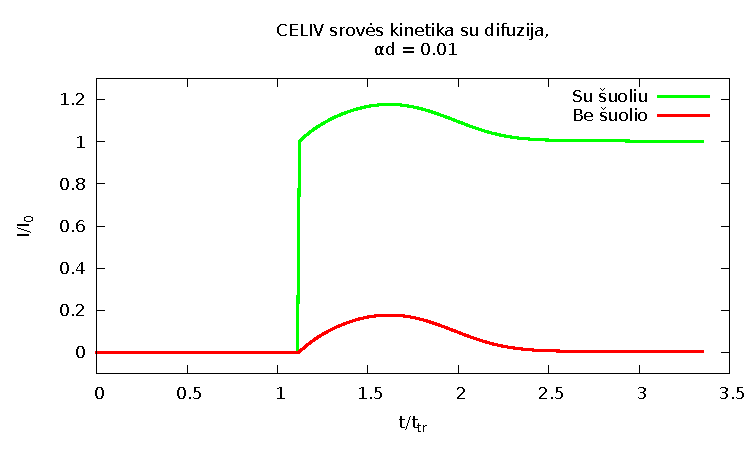
\includegraphics[width=\textwidth]{./media/pdf/jump.pdf} 
\caption{CELIV kinetikos be talpinio šuolio ir su juo, esant vienodai užlaikymo trukmei $t_{delay}$}
\label{fig:suoliai}
\end{figure}


Šios programos funkcija -- atkartoti realaus eksperimento eigą ir pateikti teorinį rezultatą, kurį galima tapatinti su realiu eksperimentu.

Realios photo-CELIV kinetikos susideda iš dviejų dalių: talpinio šuoliuko, atsirandančio dėl išorinės įtampos, prijungtos prie bandinio, ir krūvininkų ištraukimo sąlygotos kinetikos dalies \cite{juška:4946}. Šioje programoje dėl paprastumo talpinis šuoliukas nėra modeliuojamas (žr. \ref{fig:suoliai}~pav.). Jis gali būti pridedamas apdorojimo metu \(I_0 = \frac{\varepsilon \varepsilon_0 A S}{d}\).

Kinetikos atvaizduojant normuotos į srovę \(I_0\) ir į teorinę CELIV lėkio trukmę \(t_{tr} = d \sqrt{\frac{2}{\mu A}} \) \cite{juška:155202}. Čia \(A\) -- įtampos kilimo koeficientas. Visose kinetikose bus naudojama užlaikymo trukmė tarp šviesos impulso ir CELIV signalo $t_{delay}$.

\subsection{Simuliacija}

Norėdami ištirti difuzijos įtaką krūvininkų pernašai photo-CELIV atveju simuliuojame eksperimentą, kurio metu po fotogeneracijos bandinys paliekamas laikui \(t_{delay}\) atjungtas nuo išorinės grandinės, taigi jo viduje vyksta tik krūvininkų rekombinacija ir difuzija. Tokiu būdu galime atskirti stiprų pradinį difuzijos signalą nuo kitos CELIV signalo dalies.

Norėdami ištirti difuzijos įtaką krūvininkų rekombinacijos spartos matavimui, simuliuojame realų rekombinacijos spartos matavimą: keičiame \(t_{delay}\) ir sekame photo-CELIV srovės maksimumo vertės kitimą. Iš sumodeliuotų maksimumo vertės priklausomybių nuo užlaikymo trukmės galėsime nustatyti atsirandančią paklaidą dėl difuzijos.

\subsection{Sąlygos}
\label{page:params}
Bandinio ir eksperimentiniai parametrai parinkti taip, kad būtų kuo artimesni realiems.
\begin{itemize}
\item Trikampio įtampos signalo trukmė 0.1ms, įtampa kinta nuo 0 iki 1V.
\item Krūvininkų judrių santykis \(\frac{\mu_n}{\mu_p} = 1000\), taigi praktiškai juda tik vieni krūvininkai, mūsų atveju -- su neigiamu krūviu. 
\item Pasirinkti pilnai blokuojantys bandinio kontaktai, tokie, kad krūvininkai per juos negalėtų nei patekti į bandinį  nei išeiti iš jo.
\item Kur nenurodyta kitaip naudojamas šviesos intensyvumo parametras \(I_0 S \equiv L = 10^{10} \) nes su tokia verte pasiekiama soties nuo generacijos intensyvumo vertė, plačiau aprašyta \ref{page:saturation} skyrelyje.
\end{itemize}
Pavyzdinis tokios simuliacijos įvesties failas pateiktas priede \ref{app:failas}.

\subsection{Pastabos}
\label{page:specials}
\begin{itemize}
\item Visame darbe bus naudojamos srovės kinetikos be talpinio šuolio (žr. \ref{fig:suoliai} pav.).
\item Skaitmeninio modeliavimo netikslumai neleidžia skaičiuoti su be galo mažu laiko žingsniu, dėl to susidurta su efektyvia krūvininkų kiekio riba, kurią peržengus išryškėja paklaidos dėl C++ \textbf{double} kintamųjų tipo verčių netikslumo. Šią ribą apytiksliai atitinka šviesos intensyvumo parametras $L=10^{20}$. Realiai tokios vertės pasiekti neįmanoma, nes laikantis modelyje nurodytų sąlygų pirmame atomų sluoksnyje būtų generuojama $\frac{L (1-e^{-\alpha a})}{S/a^2}$ elektronų. Kai tarpatominis nuotolis $a = 2$\AA, viename atome būtų sugeneruota $800$ elektronų.
\end{itemize}

\section{Problemos}

Praeituose darbuose nustatyta, jog esant paviršinei šviesos sugerčiai $(\alpha d > 1)$ sudaromi pakankami krūvininkų pasiskirstymo gradientai, kad modeliuojamose photo-CELIV kinetikose matytųsi difuzinė srovės komponentė.
[Paveiksliukas]

Priklausomai nuo skaičiavimo būdo skiriasi difuzijos įtaka skaičiuojamam rezultatui.

Dėl atsiradusios difuzijos komponentės pakinta šie matavimų rezultatai:

\subsection{Rekombincijos matavimai}

Skaičiavimai atlikti naudojant bimolekulinės Lanževeno rekombinacijos atvejį. Suskaičiavus srovės kinetikas esant skirtingoms užlaikymo trukmėms pagal kinetikos maksimumo vertės kitimą perskaičiuotas rekombinacijos koeficientas. Jis palygintas su pradinių skaičiavimuose naudotu koeficientu.

[Ar reikia formulės?]

[Paveiksliukas] 

Pastebėta, jog atsiranda neatitinkimai tarp realaus (nustatyto) rekombinacijos koeficiento ir apskaičiuoto (virtualiai išmatuoto) koeficiento.

\subsection{Judrio matavimai}

Pagal [čia] aptartą būdą skaičiuojant krūvininkų judrį iš srovės kinetikų gaunama tokia krūvinikų judrio priklausomybė nuo užlaikymo laiko.
[Paveiksliukas]

Anksčiau panašūs rezultatai buvo aiškinami krūvininkų prilipimu. Tačiau šioje simuliacijoje krūvininkų prilipimas nėra įskaitomas, taigi egzistuoja kitos priežastys šiam kitimui.

\subsection{Skaičiavimai} 

Šitiem dalykams stebėti mes suskaičiavom tai: ... ?


\section{Rezultatai}

\subsection{Difuzijos įtaka}


\subsection{Kinetikų soties vertė}
\label{page:saturation}
\begin{figure}[h]
  \centering
	\subfloat[Logaritminė skalė]{
		\label{fig:saturation_log}
		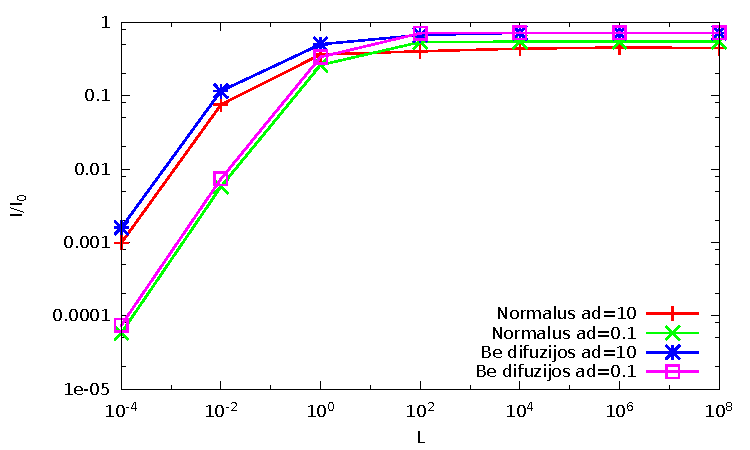
\includegraphics[width=0.5\textwidth]{./media/pdf/saturation.pdf}
		}
	\subfloat[Pusiau logaritminė skalė]{
		\label{fig:saturation_semilog}
		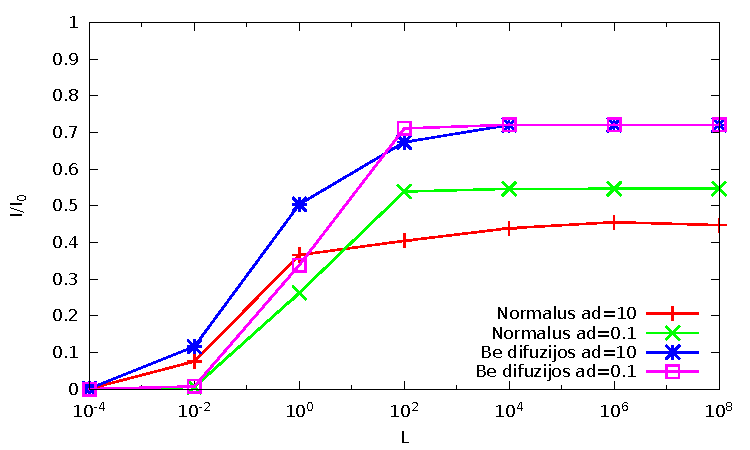
\includegraphics[width=0.5\textwidth]{./media/pdf/semilogsaturation.pdf}
		}
  \caption{Kinetikų maksimumo vertės sotinimas nuo šviesos intensyvumo, priklausomai nuo difuzijos ir sugerties profilio, esant minimaliam užlaikymui $t_{delay}$}
  \label{fig:saturation}
\end{figure}

Rekombinacijos įvertinimui naudojama srovės soties vertė, kai nėra užlaikymo laiko tarp šviesos impulso ir ištraukiančios įtampos impulso. Atlikę srovės soties skaičiavimus (žr. \ref{fig:saturation} pav.) pastebime, jog soties vertė, neįskaitant difuzijos, dėl užlaikymo laiko pakinta per pastovų dydį, nepriklausomai nuo sugerties profilio $\alpha d$. Įskaičius difuziją, srovės soties vertė ima priklausyti nuo $\alpha d$.

Iš šių rezultatų seka dvi išvados:
\begin{itemize}
\item Rekombinacijos įvertinimas pagal soties reiškinį jautrus užlaikymo laikui $t_{delay}$.
\item Veikiant difuzijai kinetikų soties vertė priklauso nuo krūvininkų sugerties profilio.
\end{itemize}

\subsection{Rekombinacijos koeficiento vertė}

\begin{figure}
  \centering
	\subfloat[Be difuzijos]{
		\label{fig:delays_nodiff}
		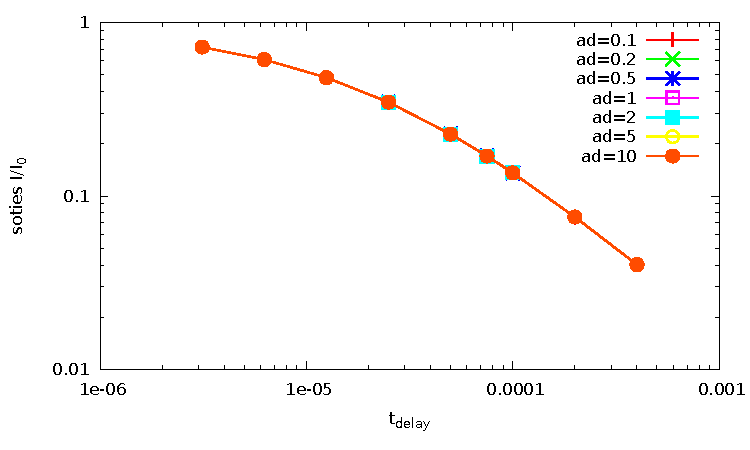
\includegraphics[width=0.5\textwidth]{./media/pdf/delays_nodiff.pdf}
		}
	\subfloat[Su difuzija]{
		\label{fig:delays_diff}
		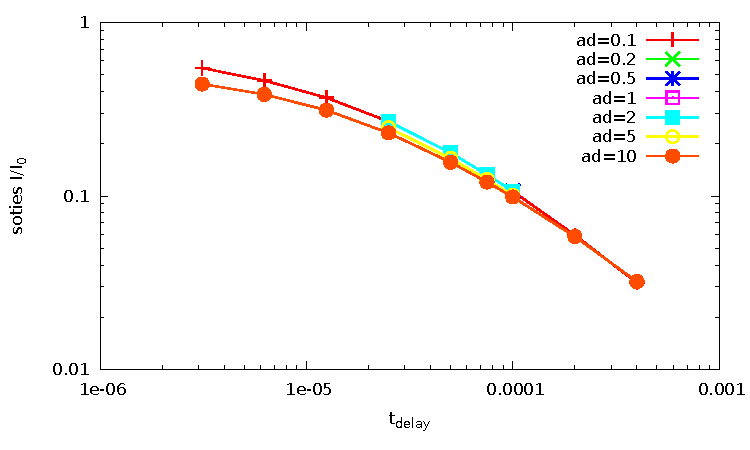
\includegraphics[width=0.5\textwidth]{./media/pdf/delays_diff.pdf}
		}
  \caption{Photo-CELIV srovės kinetikų soties vertės priklausomybės nuo užlaikymo trukmės $t_{delay}$}
  \label{fig:delays}
\end{figure}

Norėdami atmesti užlaikymo laiko įtaką kinetikos soties srovei atlikome skaičiavimus su skirtingomis užlaikymo trukmėmis, kurių rezultatai pavaizduoti \ref{fig:delays} paveiksliuke.

Pastebime, [kažkokį rezultatą]

Šie rezultatai dar kartą parodo, jog veikiant difuzijai kinetikų soties vertė priklauso nuo krūvininkų sugerties profilio.

\subsection{Judrio vertės matavimai}
Pagal šią formulę skaičiuojant krūvininkų judrį iš įsisotinusių srovės kinetikų maksimumų gaunama krūvinikų judrio priklausomybė nuo užlaikymo laiko pavaizduota \ref{fig:mobility} paveiksliuke. Anksčiau panašūs rezultatai buvo aiškinami krūvininkų prilipimu \cite{•}. Tačiau šioje simuliacijoje krūvininkų prilipimas nėra įskaitomas, taigi egzistuoja kitos priežastys šiam kitimui.

\begin{figure}
  \centering
	\subfloat[Be difuzijos]{
		\label{fig:mobility_nodiff}
		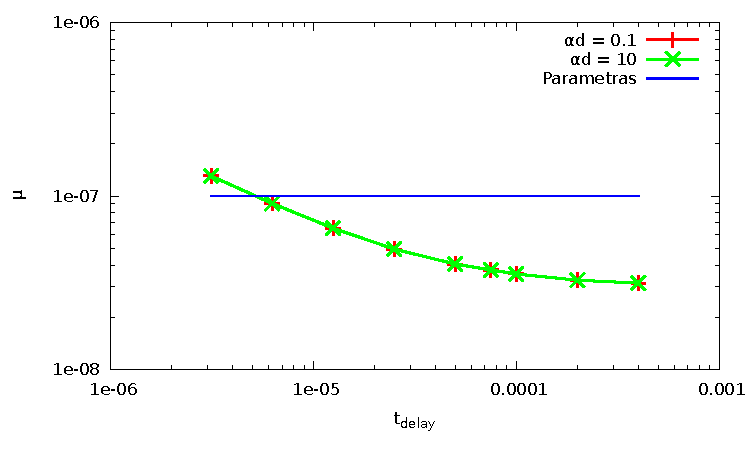
\includegraphics[width=0.5\textwidth]{./media/pdf/log_mobility_nodiff.pdf}
		}
	\subfloat[Su difuzija]{
		\label{fig:mobility_diff}
		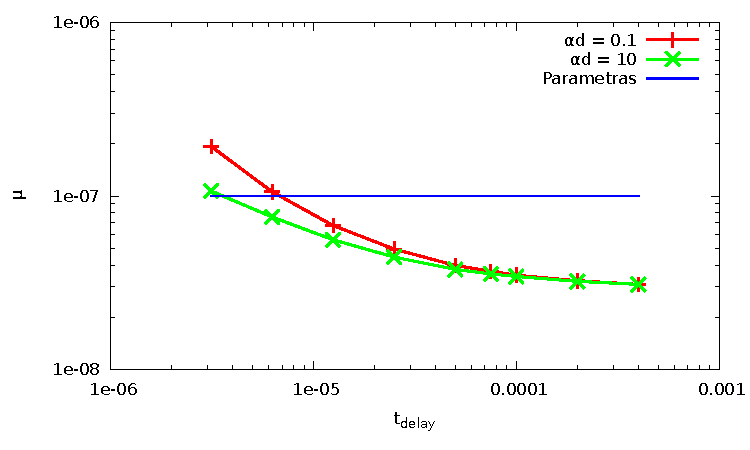
\includegraphics[width=0.5\textwidth]{./media/pdf/log_mobility_diff.pdf}
		}
  \caption{Krūvininkų judrio skaičiavimo pagal \eqref{eq:judris} formulę rezultatų priklausomybė nuo $t_{delay}$}
  \label{fig:mobility}
\end{figure}


\pagebreak
\section{Svarbiausi rezultatai ir išvados}
\begin{itemize}
\item Difuzija sumažina išmatuotą rekombinacijos koeficientą bandinyje visais tirtais atvejais, jei matavimui naudojama photo-CELIV srovės kinetikos soties vertė. Pokytis gali siekti 20-50\% priklausomai nuo krūvininkų sugerties profilio.

\item Pastebėjome, kad krūvininkų judrio matavimo rezultatai iš photo-CELIV kinetikos maksimumo padėties priklauso nuo užlaikymo trukmės. Šią priklausomybę gali sąlygoti krūvininkų kiekio kitimas \cite{juška:155202}. Tačiau įskaičius difuziją, esant $t_{delay} < t_{tr}$ judrio vertė papildomai pakinta iki 2 kartų, priklausomai nuo pradinio pasiskirstymo.

\end{itemize} 


\pagebreak
\appendix

 
\section{Paketų atsiskyrimas ir deformacija}
\label{app:negative_current}

\begin{figure}
\subfloat[\(t=0\)ms]{\label{video:1}
\centerline{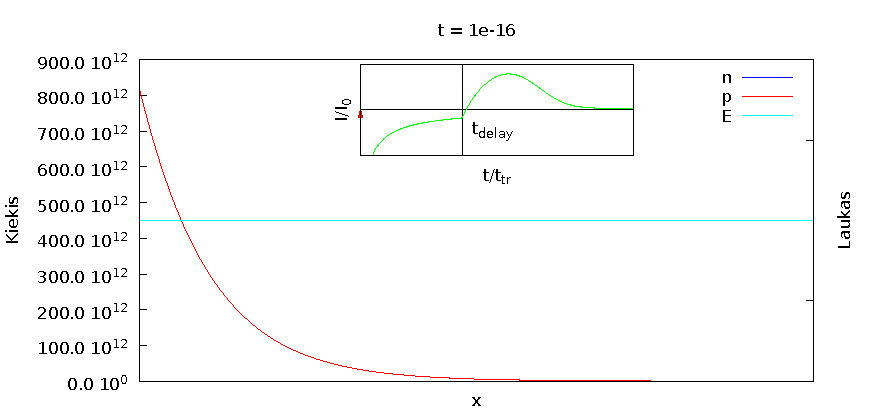
\includegraphics[height=0.28\textheight]{./media/video/00000.pdf}
}}\\
\subfloat[\(t=0.005\)ms]{\label{video:2}
\centerline{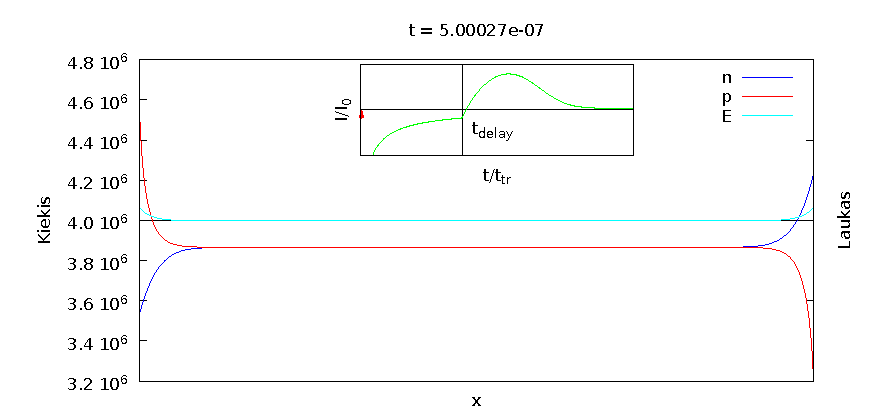
\includegraphics[height=0.28\textheight]{./media/video/00005.pdf}
}}\\
\subfloat[\(t=0.08\)ms]{\label{video:3}
\centerline{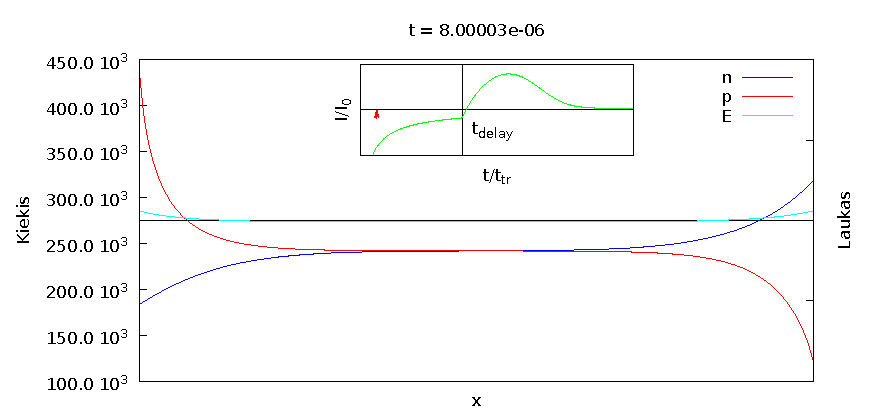
\includegraphics[height=0.28\textheight]{./media/video/00080.pdf}
}}
\caption{Simuliacijos būsenos kitimas laike}
\end{figure}

\begin{figure}
\ContinuedFloat
\subfloat[\(t=0.24\)ms]{\label{video:4}
\centerline{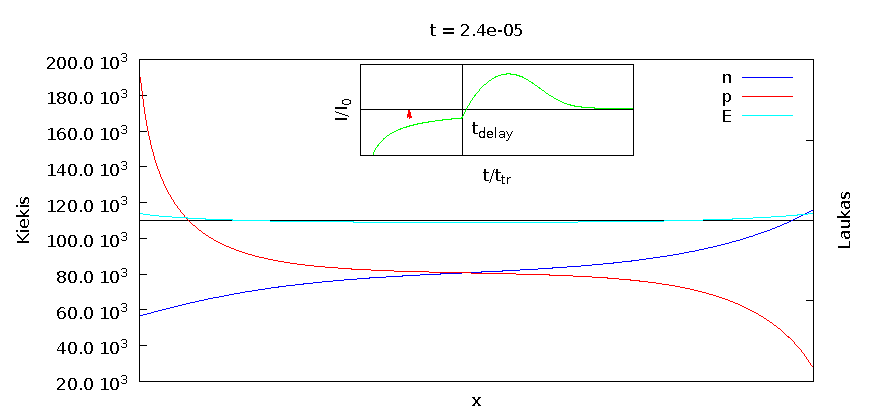
\includegraphics[height=0.28\textheight]{./media/video/00240.pdf}
}}\\
\subfloat[\(t=0.5\)ms]{\label{video:5}
\centerline{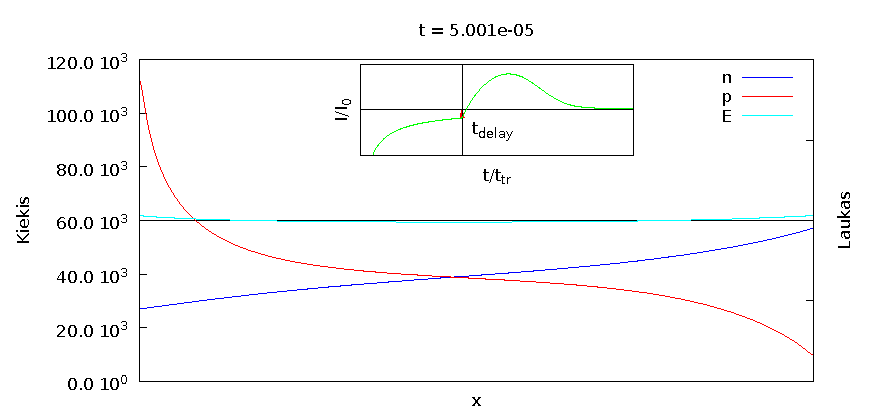
\includegraphics[height=0.28\textheight]{./media/video/00500.pdf}
}}\\
\subfloat[\(t=0.65\)ms]{\label{video:6}
\centerline{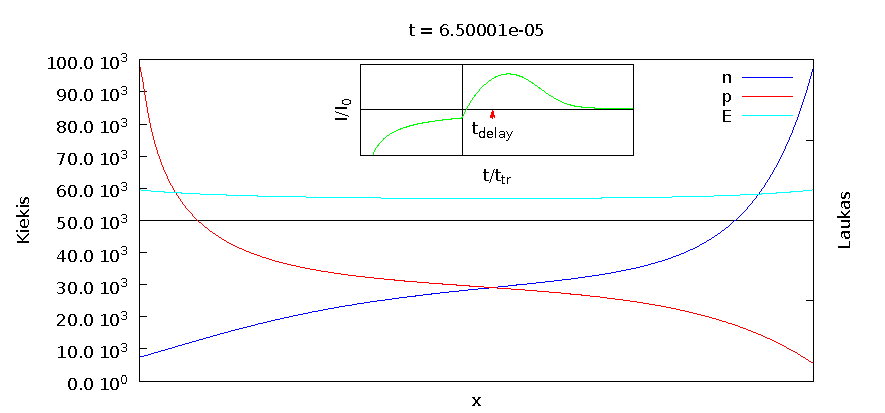
\includegraphics[height=0.28\textheight]{./media/video/00650.pdf}
}}
\caption{Simuliacijos būsenos kitimas laike (tęs.)}
\label{fig:video}
\end{figure}

Pagal darbe aprašytus simuliacijos parametrus (žr. \ref{page:params} skyrelį),kai $\alpha d = 10$, atlikti skaičiavimai, kurių rezultatų pavyzdžiai pateikti \ref{fig:video} pav.
Juose pavaizduoti krūvininkų tankių ir elektrinio lauko pasiskirstymai, skirtingais laiko momentais. Viduryje pavaizduota apskaičiuotoji CELIV kinetika, čia raudona rodyklė žymi laiko momentą, kurio metu sistemos būsena pavaizduota išoriniame paveiksliuke. Nekintanti vertikali juoda linija žymi CELIV signalo pradžią.
Matome, jog pradiniais laiko momentais (\ref{video:1}, \ref{video:2}, \ref{video:3}) krūvininkų tankių pasiskirstymai atsiskiria vienas nuo kito dėl Demberio efekto ir rekombinacijos. Tarp krūvininkų atsiranda nedidelis elektrinis laukas, žymimas žalia linija, čia juoda horizontali juoda linija žymi lauką $E=0$. Dėl elektrinio lauko atsiranda dreifo srovė. Dėl lėtesniųjų krūvininkų nejudrumo rekombinacijos sparta priklauso nuo koordinatės, taigi sukuriamas neigiamas greitesniųjų krūvininkų tankio gradientas kuris kuria difuzijos srovę. Taigi neigiamą srovę kuria difuzinė ir dreifinė komponentės. Vėliau neigiama srovė mažėja, nes krūvininkai artėja link pusiausvyros busenos. Nepasiekus pusiausvyros įjungiamas CELIV signalas ir krūvininkai traukiami prie kontaktų (\ref{video:5}, \ref{video:6}).

\section{Įvesties failo pavyzdys}
\label{app:failas}
\verbatiminput{./media/other/example.txt}



\pagebreak
\bibliography{bibliography}
\bibliographystyle{unsrt}

\pagebreak
\section*{Santrauka}
Pastaruoju metu sparčiai vystoma fotogeneruotų krūvininkų ištraukimo tiesiškai kylančia įtampa metodika (photo-CELIV), leidžianti tirti plonasluoksnių organinių darinių elektrines savybes. Šiame darbe analizuojama photo-CELIV rezultatų patikimumas, kai bandinyje pasireiškia difuzija. Tiriamas rekombinacijos spartos ir krūvininkų judrio matavimo rezultatų pokytis. Pademonstruojamos paklaidos atsirandančios dėl difuzijos skaičiuojant rekombinacijos koeficientą pagal photo-CELIV srovės kinetikos maksimumo soties vertę ir parodoma difuzijos įtaka judrio vertės skaičiavimams pagal photo-CELIV srovės kinetikos maksimumo padėtį.

\section*{Summary} 
Lately much attention is attracted to photogenerated charge carrier extraction by linearly increasing voltage (photo-CELIV) technique which allows the study of electrical properties in thin-film organic samples. This work aims to analyse photo-CELIV application in measurements of carrier mobility and recombination coeficient when diffusion is observed in the sample. The alteration of measurement results are studied. This work shows the error in recombination coeficient and carrier mobility calculations from saturated photo-CELIV current transients.
\end{document}
